\section{Sensorer}\label{sensorer}
Dette afsnit beskriver forskellige sensorer, der kan være interessant for projektet. 

\paragraph{Kamera}
Kameraet kan tage billeder og billedesekvenser i form af video optagelse.
Der er typisk to kameraer af forskellig kvalitet, hvilket bør holdes i mente.

\paragraph{Accelerometer}
Accelerometeret måler accelerationen i x,y,z akserne i et koordinatsystem som vist på \cref{analyse:accelerometer:koo}.
Accelerometret kan konceptuelt forstås som en kugle der ruller rundt i et rum hvor væggene kan måle den g-kraft de bliver påvirket med.
På \cref{analyse:accelerometer:kraft} ses dette konceptuelle rum med påvirkning fra tyngdekraften. 
Sensoren vil i dette tilfælde rapportere en g-kraft i z-aksens retning.

\begin{figure}[h]
	\centering
	\begin{subfigure}[b]{0.47\textwidth}
		\centering
		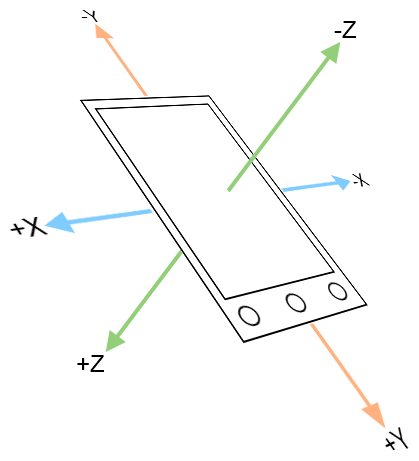
\includegraphics[width=.6\textwidth]{accelerometer-telefon}
		\caption{Koordinatsystem i forhold til telefon}
		\label{analyse:accelerometer:koo}
	\end{subfigure}
	~
	\begin{subfigure}[b]{0.47\textwidth}
		\centering
		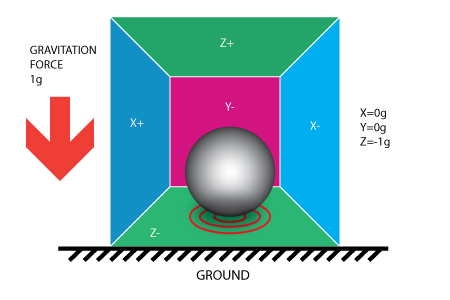
\includegraphics[width=\textwidth]{accelerometer}
		\caption{Konceptuel tegning af et accelerometers virkemåde. Illustration fra \cite{accelerometer}}
		\label{analyse:accelerometer:kraft}
	\end{subfigure}
	\caption{}
	\label{accelerometer}
\end{figure} 

\paragraph{GPS}
GPS sensoren giver en lokation som koordinater bestående af: breddegrad, længdegrad og en pejling.
Ved at differentiere positionen ift. tid kan man blive oplyst om hastigheden og ved at differentiere igen kan man blive oplyst om accelerationen.
Denne sensor er dog ofte utilgængelig når enheden er indendørs, da de signaler der bruges til GPS positionsbestemmelse ikke kommer ind i de fleste bygninger.

\paragraph{Mikrofon}
Mikrofonen kan optage omgivelserne ved at konvertere akustisk lyd til elektriske signaler. Kvaliteten og følsomheden af denne kommer an på selve telefonen, idet at der er mange forskellige mikrofoner som bruges i telefoner. 

\paragraph{Lyssensor}
Lyssensoren kan måle belysningsstyrken på en flade i lux. Det er intensiteten af lyset der kan måles på en flade.

\paragraph{Pulsmåler}
Pulsmåleren måler pulsen i hjerteslag per minut ved enten en elektrisk puls igennem et ledende materiale på huden, eller via en optisk sensor man sætter fingeren på.
Den mest præcise måling fås hvis sensoren sidder spændt omkring brystet, mens sensorer der måler enten på håndleddet eller fingeren er mindre præcise \cite{burke1998precision}.

\paragraph{Galvanisk Hud Respons}
Galvanisk hud respons sensoren giver adgang til data om hvor god hud er til at lede strøm, huden leder strøm bedre jo mere den sveder, og giver derfor også data om hvor meget den sveder.